\subsection{Generating Text with Recurrent Neural Networks \cite{Martens2011}}

This paper proposes a new variant of \emph{Recurrent Neural Network (RNN)} called \emph{Multiplicative Recurrent Neural Network (MRNN)}, and demonstrates its power by applying it to character-level language modeling tasks. Specifically, the paper will use the MRNNs to predict the next character in a stream of text.

The standard RNN is formalized as follows: Given a sequence of input vectors $(x_1, ..., x_T)$, the RNN computes a sequence of hidden states $(h_1, ..., h_T)$ and a sequence of outputs $(o_1, ..., o_T)$ by iterating the following equations:
\begin{eqnarray}
h_t &=& tanh(W_{hx}x_t + W_{hh}h_{t-1} + b_h)\\
o_t &=& W_{oh}h_t + b_o
\end{eqnarray}

In the standard RNN the current input $x_t$ is first transformed via the weight matrix $W_{hx}$ and then contributes \emph{additively} to the hidden state, while the basic idea of MRNN is to allow the current input determine the entire hidden-to-hidden matrix ($W_{hh}$). Before going further, it is worthy to explain the motivation of this approach.

\begin{figure}[htbp]
  \centering
  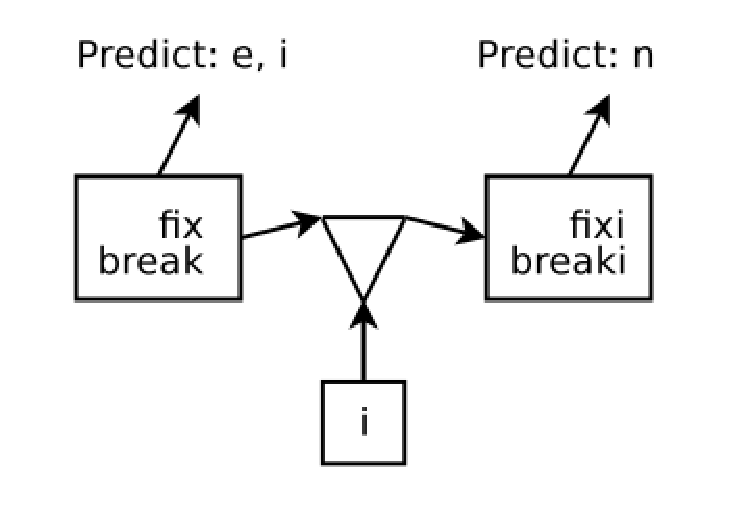
\includegraphics[width=.5\linewidth]{8_1_mrnn}\\
  \caption{A example that requires multiplicative connection}\label{fig:mrnn}
\end{figure}

For example in Figure \ref{fig:mrnn}, the character string ``ing'' is quite probable after ``fix'' and also quite probable after ``break''. If the hidden state vectors of the two words share a common concept of the stem of a verb, then there is a common representation to allow the character ``i'' to produce ``n''. Any evidence alone (verb stem or character ``i'') is not sufficient to make the prediction, and adding the weight additively is intuitively not a good strategy.

Based on the above analysis, in MRNN the update rule of hidden state vectors is changed to:
\begin{eqnarray}
h_t &=& tanh(W_{hx}x_t + W^{(x_t)}_{hh}h_{t-1} + b_h)
\end{eqnarray}
Here $W_{hh}$ is replaced with $W_{hh}^{(x_t)}$, allowing each character to specify a different hidden-to-hidden weight matrix.

The above scheme has a major drawback, which is that the storage required for $W_{hh}^{(x_t)}$ becomes prohibitive when the dimensionality of $x_t$ is even moderately large. The paper overcomes this problem by factoring $W_{hh}^{(x)}$ with three matrices $W_{fx}, W_{hf}$ and $W_{fh}$:
\begin{eqnarray}
W_{hh}^{(x_t)} = W_{hf} \cdot diag(W_{fx}x_t) \cdot W_{fh}
\end{eqnarray}
As a result, the updating rules can be represented as:
\begin{eqnarray}
f_t &=& diag(W_{fx}x_t) \cdot W_{fh}h_{t-1}\\
h_t &=& tanh(W_{hf}f_t + W_{hx}x_t)\\
o_t &=& W_{oh}h_t + b_o
\end{eqnarray}

In the experimental section, the paper makes comparison study with the \emph{sequence memorizer}  and \emph{PAQ}  methods. It is reported that MRNN achieves lower \emph{bits per character (bpc)} than the sequence memorizer but higher than PAQ (lower bpc implies better performance). The second part of experiment is to evaluate different methods with the \emph{debagging problem}, which is to convert a bag of words into a meaningful sentence. MRNN recovers the correct ordering 34\% of the time, which is higher than the memorizer (27\% of the time). Finally and most interestingly, the proposed neural network is used to generate sentence in character level, given a beginning of the sentence. For example, when initialized with the phrase ``The meaning of life is'', the MRNN generates the following sentence:

\begin{small}
The meaning of life is the tradition of the ancient human reproduction: it is less favorable to the good boy for when to remove her bigger. In the show's agreement unanimously resurfaced. The wild pasteured with consistent street forests were incorporated by the 15th century BE. In 1996 the primary rapford undergoes an effort that the reserve conditioning, written into Jewish cities, sleepers to incorporate the .St Eurasia that activates the population. Mar??a Nationale, Kelli, Zedlat-Dukastoe, Florendon, Ptuos thought is. To adapt in most parts of North America, the dynamic fairy Dan please believes, the free speech are much related to the...
\end{small}
